\section{Strategies and Concepts}
\label{sec:strategies}

\subsection{Single Player}
After identifying four tenets for guiding organism development, we attempted to build strategies that would account for the variable elements inherent to the Organisms board, including:

\begin{itemize}
\item	p--probability of spontaneous food appearance
\item	q--probability of food doubling
\item	v--energy consumed by moving or reproducing
\item	u--energy per unit of food
\item	M--maximum energy per organism
\item	K--maximum food units per cell
\item	m,n--board size
\end{itemize}

The first strategy we developed aimed to qualify the third insight: stay still when advantage of moving is unclear.  To do this, we planned to develop thresholds for each behavior, effectively quantifying the relative value of moving, reproducing, and staying put.  A mathematical approach quickly revealed that these thresholds would be functions of p and q.

Having found this, we elected to design an organism behavior that would communally measure these variables.  To do this, we developed the Talker, an organism which observed board conditions and relayed those conditions, along with an indicator of the data quality, back to the other organisms on the board.


\subsubsection{Talker}
\TODO{[DESCRIBE STRATEGY IN-DEPTH HERE]}

The talker was effectively a proof-of-concept--while it did successfully relay board conditions, albeit only approximately, we soon realized that a pattern-based strategy was better suited for a single-player board.

This realization became apparent when trying to calculate the maximum sustainable energy of the board. To calculate this, we assume that each organism is adjacent to exactly one farm.  In this case, there are 355 organisms under normal conditions:
\begin{verbatim}
	Total number of cells			=	400
	Number of Farms	=	400 / 9 	= 	45
	Number of Organisms = 	400 - 45	= 	355
\end{verbatim}

If this is the case, and each organism can maintain maximum energy, the maximum sustainable board energy is 177,500
\begin{verbatim}
	Total Number of Organisms * Max Energy Per Organism = 177,500
\end{verbatim}

\subsubsection{PatternMaker}
Upon realizing this theoretical maximum, we began to approach the problem differently: rather than problem mimicking biological behavior, this became a packing problem, or an environment that had to be most efficiently utilized.  Rather than attempting to hardcode behaviors into the organisms, we gave each one of six specific roles.  These role were differentiated on two counts:
\begin{enumerate}
\item Each role only reproduced children of one or two other specific roles in a specific direction, and
\item Each role only ��harvested�� the farm at a specific, unique point during a 32-turn cycle.
\end{enumerate}

Each organism had a cyclical concept of a turn number which was incremented every turn.  This, rather than energy thresholds, determined when behaviors would happen.  PatternMaker organisms on their own are very dumb, but collectively, they do an excellent job of maximising the resources on the board.

\begin{figure}[htf]
\centering
  % Requires \usepackage{graphicx}
  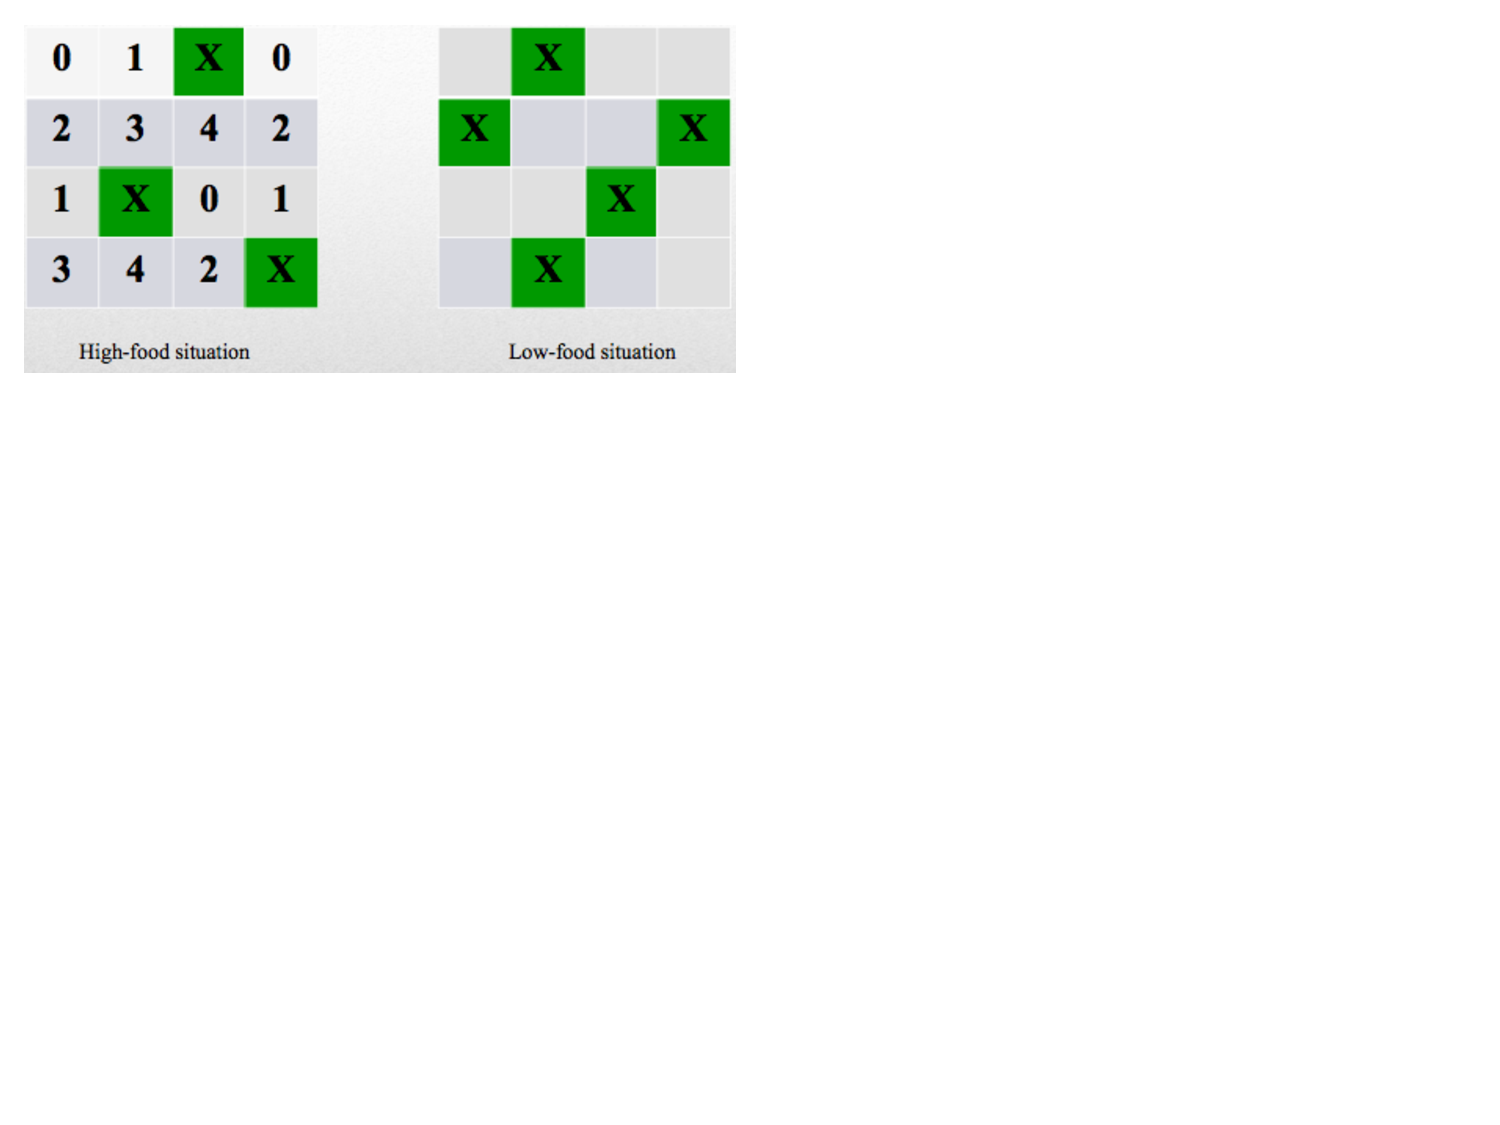
\includegraphics[trim=10mm 130mm 135mm 10mm]{figs/high-low-food.pdf}\\
  \caption{PatternMaker harvesting patterns in high- and low- food situations}
  \label{fig:high-low-food}
\end{figure}


Another PatternMaker organism was developed to deal with low-food situations.  This patternmaker relied on the same concept described above, but instead allowed each organism to be orthogonal to two farms instead of one.  This resulted in separated, diagonal patterns rather than L-shaped ones (see Figure~\ref{fig:high-low-food}).

An attempt was made to reconcile the Talker and PatternMaker strategies.  The goal was to identify whether the board has a high or low q value and then generate the corresponding pattern.  However, this proved to be ineffective: even after identifying a data-robustness level sufficient to make a patterning decision, patterning proved ineffective because of the residual Talker organisms left on the board. 

\subsubsection{Surviving Mode}
One thing we noticed is that for harsh environment(p = 0.1\%), the
organism will easily extinct if moving around too much, especially at
the beginning of game.  However, if we are able to let the food to
grow for a while, the board will become abundant, which then allows
the organism to make some move and maximize total power.  Basically,
we attempt to help our organism \textit{Survive} the beginning couple
hundred rounds(Stage One) and switch to energy miximizing mode(Stage
Two). Note that the surviving mode is just one layer put at the
beginning of the game. At some point(details in Implementation), when
organism enters stage two, \textit{any} algorithm for maximizing energy could
be invoked. The two stages are totally decoupled.

\textbf{Move or stay.}  During this surviving mode, apparently,
reproduce is not a good action.  The energy spliting makes the
origanism weak and cost of stayput will doubled.  The question
remained to be whether the organism should just stay, waiting for food
to appear in the neighbor cells or move around to explore food. We
answer this question by introducing a probabilistic analysis over the
benefit of moving or stay.  More specifically, we will calculate the
probability of finding food when you move and compare it with the
probablity of finding food if those energy are used to stayput and
wait, so as to determine the best action in each round.

\textbf{Eat or wait.} The idea above is focusing on finding one food.
But once a food is found in neighbor cell, shall the organism just go
ahead and eat it or wait for as long as it can. Our answer is the
later, based the following three reasons.
\begin{enumerate}
\item This is single player mode, no one will appear and rob the food
  away.
\item The goal of this stage is to survive the beginning harsh
  environment, waiting is more suitable to this.
\item The expectation of food on that cell grows exponential to the
  time you wait(more details in Implementation).
\end{enumerate}



\subsection{Multiple Player}
\subsubsection{Flood}
Our multiple-player organism is named \textit{Flood}, which comes from the flooding behavior of the strategy. 

\textbf{Generations.} We defined three \textit{generations} for this strategy, determined by the amount of energy left,
playing different roles for the whole organism family.
\begin{itemize}
\item[Gen 0:] Aggressively move, rob food and reproduce. (E.g., the very initial organism(the mother).)
\item[Gen 1:] Mildly expand, search food, reproduce if energy is high enough.
\item[Gen 2:] Stay quietly, only move if food around. If find more than one friend around, try moving away and be sparse looking.
\end{itemize}
Generation $0$ is attempting to spread out as fast as possible, find more food, cover more ground.
Generation $1$ is in between, not so aggressive, but also not really quiet.
Generation $2$ will stay for most of the time, attempting to defend the zone covered and absorb resource on it.

\textbf{Stay Sparse.} We want to highlight our strategy for generation $2$ of being spare here. 
We believe that we are the very first group to actually point this out.
There are lots of advantages of such action.
\begin{enumerate}
\item Use less organism to cover more places.
\item The empty space in between can be treated as some sort of farm, making the coverage more sustainable.
\item Each organism has a chance to see more empty block around, provides it more chance to survive and hold the area. 
\end{enumerate}

\textbf{Genetic Mutation.} The key trick of this player is that, we enable mutation for the organisms based on the energy it has. 
For instance, if a generation $2$ organism finds a cell with lots of food, then it has enough energy to be aggressive and will thus mutate to generation 0.
Such strategy allows the family to form a self-balanced ecosystem. 
When organisms have low energy, they will stay still and try to stay as long as possible and wait for chance.
When some organism has high energy, they will attempt to expand, use the extra energy to cover more ground and to suffocate the enemies. 

\textbf{Block Enemy.} For any generation, if observe enemy in neighbor cell, it will stay still, attempt to block the action of that enemy and only move if observing food.
